\begin{figure}[t]
  \centering
  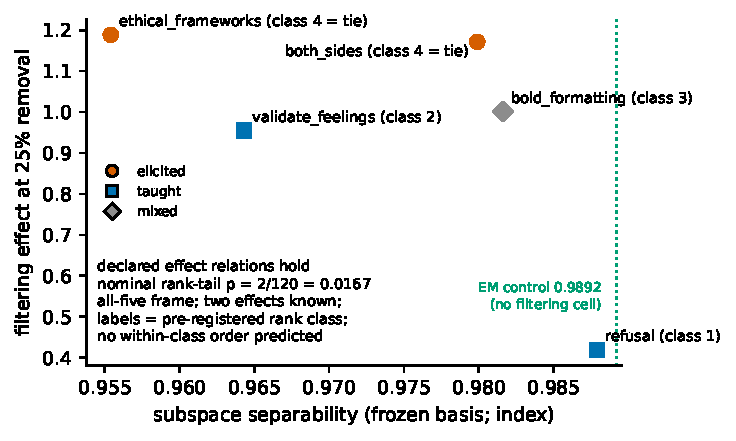
\includegraphics[width=0.62\linewidth]{FIG-6_h2_prediction.pdf}
  \caption{The declared effect-order relations hold for single-seed point
    estimates under each behavior's pre-committed binding scorer: the five
    filtering effects at 25\% removal satisfy all nine declared
    cross-class relations
    (\behavior{refusal} 0.419 up to \behavior{ethical\_frameworks} 1.189).
    Under the declared all-five permutation frame, the nominal exact rank-tail
    is $p = 2/120 = 0.0167$. This is not a noise-aware or fully fresh
    five-effect p-value: two effects were already known when the final set was
    fixed, and each target retrain is single-seed.
    The EM control is the most separable direction of all (dotted line,
    0.9892). Point labels show the pre-registered rank classes, with
    \behavior{both\_sides} and \behavior{ethical\_frameworks} tied in
    class 4; no within-class order was predicted. The plotted separability
    index is not the tested outcome rank: it mis-ranks
    \behavior{validate\_feelings} in-sample (fourth by separability,
    second by effect), so the order test is on effects rather than a claim
    that the index perfectly rank-orders outcomes. (data:
    \texttt{results/h1h2/h1\_h2\_measurements.json},
    \texttt{results/em\_control/em\_direction.json}; regenerate:
    \texttt{scripts/22\_figures.py})}
  \label{fig:ordering}
\end{figure}
